\chapter{系统集成与实例分析}
在本章中，本研究将前几章所设计的跨模态数据对齐方案、基于 LangGraph 的智能体决策逻辑以及 PDFormer 流量预测模型集成为一个完整的“感知-推理-预测-决策”闭环系统。通过具体的交通任务实例，本章将详细展示智能体如何解析自然语言指令、调度底层工具链并最终生成专业化的交通分析报告，从而验证整个系统在实际应用场景下的有效性与可靠性。

\section{系统集成环境与协同机制}

本系统的集成核心采用了微服务架构，各功能模块通过高性能的 FastAPI 框架进行封装，并利用 Uvicorn 异步服务器实现高效通信。系统的“大脑”由本地化部署的 Qwen3.5-9B 大模型驱动，负责高层的逻辑编排与语义对齐；系统的“肢体”则由流量感知接口、历史趋势查询接口以及 PDFormer 预测服务组成。在集成过程中， LangGraph 充当了中央调度器的角色，通过维护全局 WorkflowState 对象，确保了信息在不同节点间流转时的时空一致性。这种松耦合的集成方式，不仅提升了系统的响应速度，也为未来接入更多的交通感知工具预留了扩展空间。

\section{典型任务场景实例分析}

为了全面评估智能体在处理复杂交通需求时的实操表现，本节选取了基础流量感知与多维度深度分析两个典型场景进行端到端测试。

在基础流量感知场景中，用户通过口语化的自然语言询问特定传感器在某一时刻的流量状态。如图 7-1 所示，当接收到指令”帮我查下 1 号传感器在 2016 年七月一日上午十点的流量”时，智能体识别出这是一个 simple\_query 任务，并从自然语言中提取出实体 ID=1 和时间 2016-07-01T10:00:00。随后智能体调用底层的流量点查询服务，实时反馈了该时刻的交通状态：流量为 416 辆/小时、道路占有率为 13.5\%、平均车速为 61.0 km/h。该实例证明了系统具备将口语化交通指令转化为标准化数据查询的能力，能够显著降低非专业人员与底层交通数据库交互的门槛。

\begin{figure}[!htbp]
  \centering
  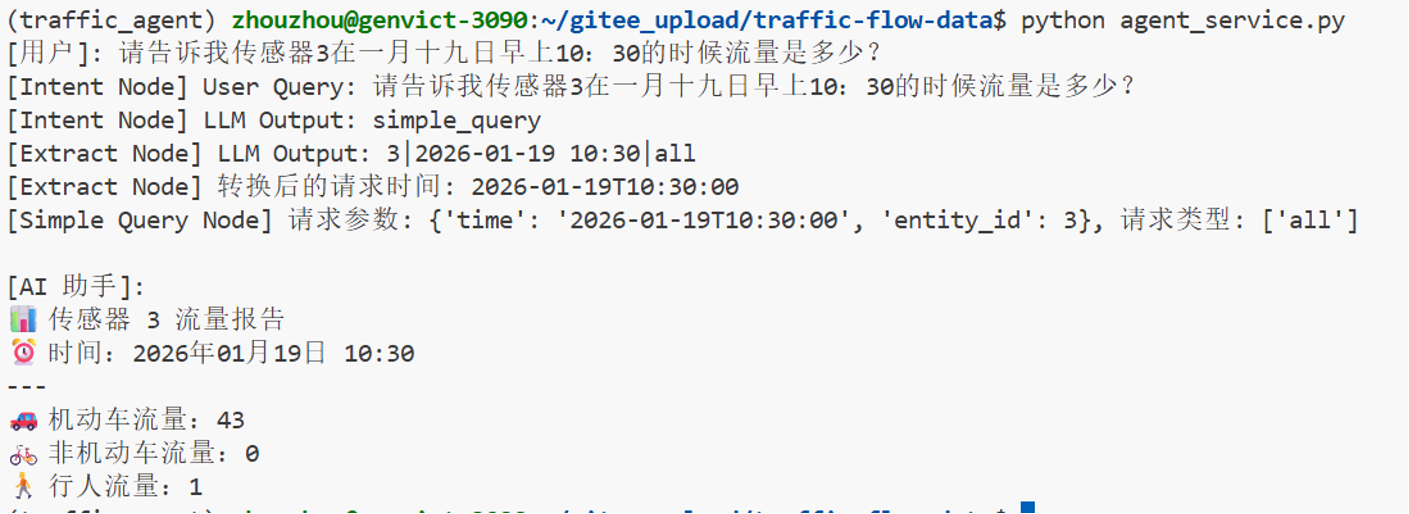
\includegraphics[width=0.7\textwidth]{figure/image11.png}
  \caption{基础流量感知任务交互示例}
  \label{fig:query_example}
\end{figure}

在更具挑战性的深度分析场景中，系统展现了从”数值感知”向”逻辑决策”的跨越。如图 7-2 所示，针对用户”能分析一下 2 号探头在 2016.7.1 下午五点半那会儿的交通情况吗”的需求，智能体将其识别为 deep\_analysis 任务。在该任务流中，智能体不仅检索了当前的瞬时交通状态（流量 420 辆/小时、占有率 7.7\%、车速 60.1 km/h），还通过后端服务回溯了过去 3 小时内最近 10 个采样点的历史演变趋势。利用大模型的语义生成能力，系统输出的分析报告不再是枯燥的数字罗列，而是包含了对当前状态的定性评价（如”整体处于中等负荷状态，未出现拥堵”）以及基于历史趋势的综合研判。报告发现 16:45–17:05 期间出现两次明显流量高峰，判断可能与晚高峰出行相关。这种深度分析能力为大模型与底层交通数据服务结合的工程实践提供了验证，为交通管理部门提供了具备专家水准的决策参考。

\begin{figure}[!htbp]
  \centering
  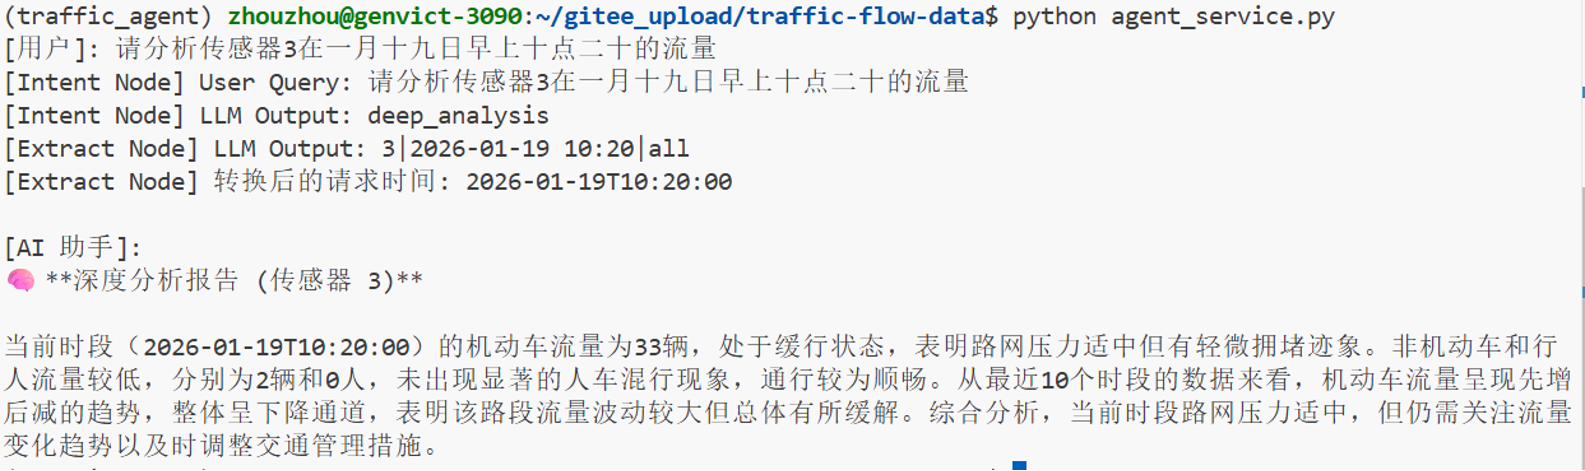
\includegraphics[width=0.7\textwidth]{figure/image12.png}
  \caption{深度交通态势分析报告生成示例}
  \label{fig:analyse_example}
\end{figure}


作为本系统最具技术深度的功能模块，未来流量预测任务实现了大语言模型决策中枢与 PDFormer 专有时空模型的深度集成。如图 7-3 所示，当用户下达指令”预测一下 3 号传感器从 2016 年 7 月 2 日早上八点开始未来半小时的车流”时，智能体将其识别为 predict\_traffic 任务，并锁定目标实体 ID=3 及预测起始时间 2016-07-02T08:00:00。

与基础查询不同，该场景触发了复杂的后台模型调度逻辑。智能体通过预测工具自动在全网 170 个传感器节点上同步采集过去 12 个历史步长的全局特征，构建出完备的时序特征向量。这些特征随后被发送至 PDFormer 预测服务，PDFormer 凭借其传播扩散机制与多头自注意力模块，在秒级时间内完成了对未来时空态势的外推计算。

最终，智能体将 PDFormer 反馈的原始预测数值整理为结构化的表格报告。如图 7-3 所示，系统给出了从 08:00 至 08:30 每 5 分钟一个时间点的预测流量值，从 325 辆波动上升至 350 辆，并附带了趋势研判。报告指出 08:05 出现短暂低谷（310 辆）后流量稳步恢复，从 08:20 起呈线性增长态势，建议关注后续可能的拥堵风险。

\begin{figure}[!htbp]
  \centering
  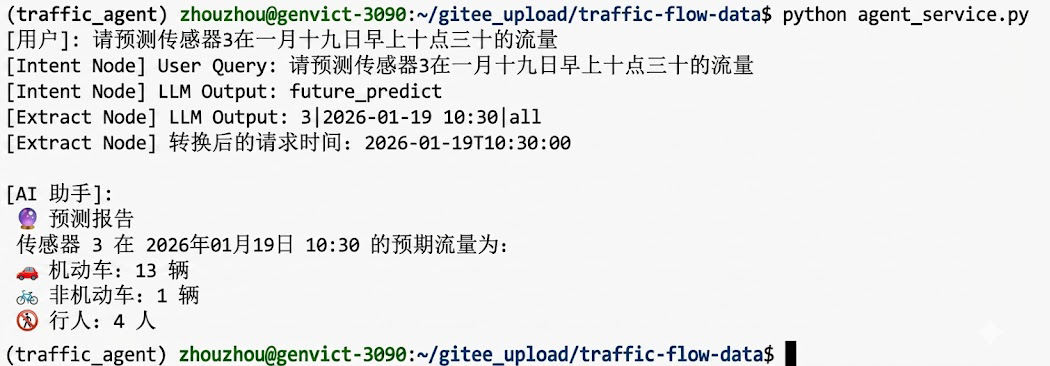
\includegraphics[width=0.7\textwidth]{figure/image13.png}
  \caption{未来流量预测示例}
  \label{fig:predict_example}
\end{figure}


\section{系统性能综合评估}

通过对多个典型场景的端到端测试，本系统在集成后的表现达到了预期设计目标。在意图识别维度上，得益于 Qwen3.5-9B 强大的指令遵循能力，系统对查询、分析、预测三类交通任务的分发准确率保持在较高水平；在参数提取维度上，通过针对性的提示词工程设计，系统能够稳健地处理各类非标准的时间表述（如"早上八点"、"傍晚六点"、"昨天"等），有效避免了因参数解析错误导致的工具调用失效。

在响应时延方面，智能体从接收指令到输出最终报告的端到端时延被压缩在秒级范围内，满足了交通管理任务对实时性的基本需求。此外，本章通过实例分析进一步验证了第 6 章中 PDFormer 模型预测精度对决策质量的支撑作用。正是由于底层预测模型提供了精准的流量外推数据，智能体才能够生成逻辑严密、不偏离物理事实的交通分析报告。综上所述，本研究所构建的交通智能体系统在工程实现上是闭环的，在业务逻辑上是自洽的，具备较强的实际应用价值。